\documentclass[hyperref={pdfpagelabels=false}]{beamer}
\usepackage{lmodern}
\usetheme{Singapore}

\makeatother
\setbeamertemplate{footline}
{
  \leavevmode%
  \hbox{%
  \begin{beamercolorbox}[wd=.2\paperwidth,ht=2.25ex,dp=1ex,center]{author in head/foot}%
    \usebeamerfont{author in head/foot}\insertshortauthor
  \end{beamercolorbox}%
  \begin{beamercolorbox}[wd=.8\paperwidth,ht=2.25ex,dp=1ex,center]{title in head/foot}%
    \usebeamerfont{title in head/foot}\insertshorttitle\hspace*{3em}
    \insertframenumber{} / \inserttotalframenumber\hspace*{1ex}
  \end{beamercolorbox}}%
  \vskip0pt%
}
\makeatletter

\usepackage{graphicx} % Allows including images
\usepackage{booktabs} % Allows the use of \toprule, \midrule and \bottomrule in tables
\usepackage{amssymb}
\usepackage{amsmath}
\usepackage{amsmath,amssymb,amstext}
\usepackage{algorithm}
\usepackage{algorithmic}


%----------------------------------------------------------------------------------------
%	TITLE PAGE
%----------------------------------------------------------------------------------------

\title[Optimization: Methods and Techniques]{Optimization: Methods and Techniques} % The short title appears at the bottom of every slide, the full title is only on the title page

\author{Yichen ZHANG} % Your name
\institute[uWaterloo] % Your institution as it will appear on the bottom of every slide, may be shorthand to save space
{
University of Waterloo \\ % Your institution for the title page
\medskip
\textit{yichen.zhang@uwaterloo.ca} % Your email address
}
\date{\today} % Date, can be changed to a custom date

\AtBeginSection[]{
\begin{frame}
\begin{center}
\begin{beamercolorbox}[sep=8pt,center]{part title}
\usebeamerfont{part title}\insertsection
\end{beamercolorbox}
\end{center}
\end{frame}
}

%\AtBeginSubsection[]{
%\begin{frame}
%\begin{center}
%\begin{beamercolorbox}[sep=8pt,center]{part title}
%\usebeamerfont{part title}\insertsubsection
%\end{beamercolorbox}
%\end{center}
%\end{frame}
%}

\begin{document}

\begin{frame}
\titlepage % Print the title page as the first slide
\end{frame}

\begin{frame}
\frametitle{Overview} % Table of contents slide, comment this block out to remove it
\tableofcontents % Throughout your presentation, if you choose to use \section{} and \subsection{} commands, these will automatically be printed on this slide as an overview of your presentation
\end{frame}

%----------------------------------------------------------------------------------------
%	PRESENTATION SLIDES
%----------------------------------------------------------------------------------------
\section{Trust-Region, Simulated Annealing and Smoothing Techniques}
\subsection{Trust-Region Method}

%------------------------------------------------

\begin{frame}
\begin{itemize}
\frametitle{Trust-Region Method}
\item A trust-region method defines a region around the current point within which the model is trusted to be an adequate representation of the objective function, and then solve the minimization problem of the model in this region.
\item Taylor's Theorem underpins most unconstrained minimization methods, and this is certainly true for trust region methods. If f is twice continuously differentiable then at $x_k\in \mathbb{R}^n$
\begin{equation}
f(x_k+s)=f(x_k)+\triangledown f_k^Ts+\frac{1}{2}s^T\triangledown ^2f_ks+o(||s||^2)
\end{equation}
\end{itemize}
\end{frame}

%------------------------------------------------

\begin{frame}
\begin{algorithm} [H]
\caption{Trust Region Method (TRM)}
\begin{algorithmic} 
\STATE 1. Solve TRS for $s_k$
\STATE 2. Adjust $\Delta_k$
\STATE 3. Update $x$
\end{algorithmic}
\end{algorithm}
 The trust region subproblem at $x_k$ is:
\begin{equation}
min\left\lbrace \triangledown f_k^Ts+\frac{1}{2}s^T\triangledown^2f_ks: ||s||\leq \Delta_k\right\rbrace
\end{equation}
\end{frame}

%------------------------------------------------

\begin{frame}
\begin{figure}
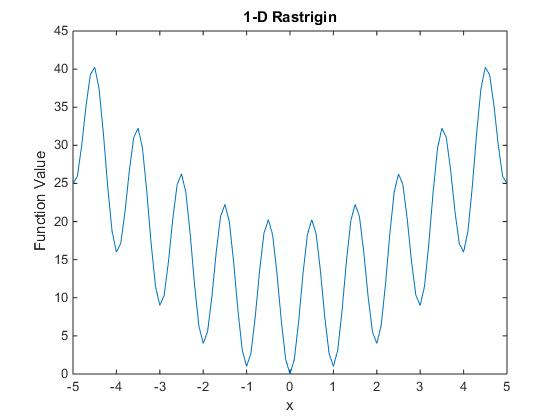
\includegraphics[scale=0.4]{1DRast.jpg}
\caption{1-D Rastrigin. $f=10+x^2-10\cos(2\pi x)$}
\end{figure}
\end{frame}

%------------------------------------------------

\begin{frame}
\begin{figure}
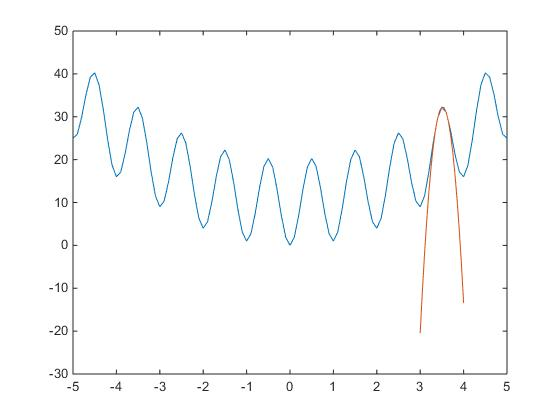
\includegraphics[scale=0.4]{1DRast3.jpg}
\caption{TRM, First Step, $x_0=3.5$, $\Delta=0.5$}
\end{figure}
\end{frame}

%------------------------------------------------

\begin{frame}
\begin{figure}
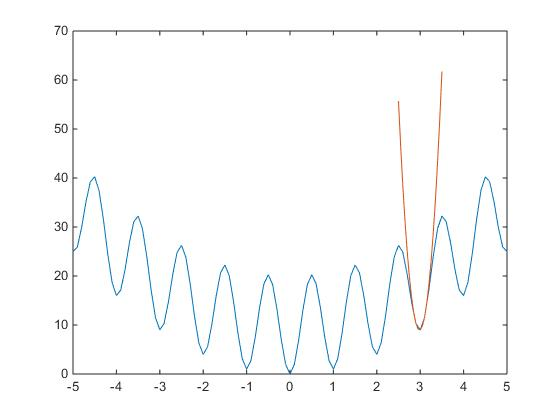
\includegraphics[scale=0.4]{1DRast2.jpg}
\caption{TRM, Second Step, $x_1=3$, $\Delta=0.5$}
\end{figure}
\end{frame}

%------------------------------------------------

\begin{frame}
\frametitle{Summary}
\begin{itemize}
\item Trust-Region method can find the (local) optimum in a few steps and a short time.
\item It will probably be a local optimum.
\item We need the gradient and Hessian.
\end{itemize}
\end{frame}

%------------------------------------------------
\subsection{Simulated Annealing}
%------------------------------------------------

\begin{frame}
\frametitle{Simulated Annealing}
\begin{itemize}
\item<1-> Unlike the traditional iteration algorithm which only accept the downhill move, simulated annealing allows perturbation to move uphill in a certain way.
\item<1-> The advantage to accept uphill move is we may escape from the local optima and find a better answer. Traditional algorithm for solving optimization problem may be trapped in the region near the start point and can not escape from it.
\end{itemize}
\end{frame}

%------------------------------------------------

\begin{frame}
\begin{figure}
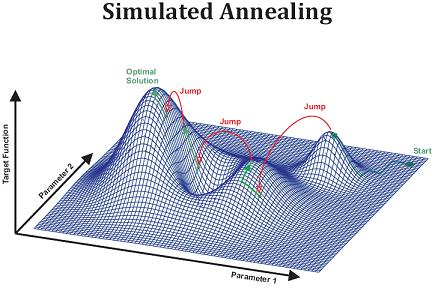
\includegraphics[scale=0.7]{sajump.jpg}
\caption{Simulated Annealing}
\end{figure}
\end{frame}

%------------------------------------------------

\begin{frame}
\begin{algorithm} [H]
\caption{Simulated Annealing at Temperature $T$}
\begin{algorithmic} 
\STATE $M$ = number of moves to attempt.
\FOR { $ m =1\ \mbox{to} \ M$ }
\STATE  Generate a new neighbouring solution, evaluate $f_{new}$.
\IF{ $f_{new} < f_{old}$} 
\STATE \emph{(downhill move: accept it)}
\STATE Accept this new solution. 
\ELSE 
\STATE  \emph{(uphill move: accept maybe)}
\STATE Accept with probability $P(T)$. 
\ENDIF
\ENDFOR
\end{algorithmic}
\end{algorithm}
\end{frame}

%------------------------------------------------

\begin{frame}
\begin{figure}
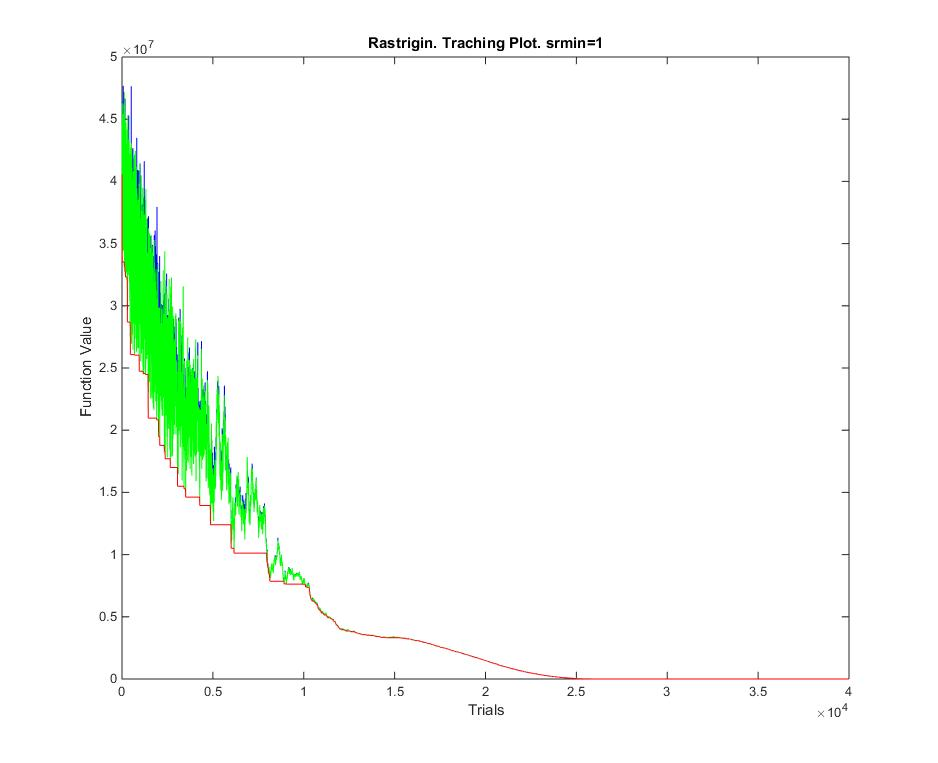
\includegraphics[scale=0.25]{srmin1.jpg}
\caption{Simulated Annealing}
\end{figure}
\end{frame}

%------------------------------------------------

\begin{frame}
\begin{itemize}
\item The simulated annealing procedure is the first phase. After that we use trust-region or some other local search technique with start point(s) from the first phase.  
\end{itemize}
\end{frame}

%------------------------------------------------

\begin{frame}
\frametitle{Summary}
\begin{itemize}
\item Theoretically, simulated annealing is a global optimum search technique and it can find the global optimum in an (infinite) time. 
\item It does not require any gradient information, just the function value.
\item The number of evaluation of $f(x)$ may be very huge.
\item All the parameters affect the performance.
\end{itemize}
\end{frame}

%------------------------------------------------
\subsection{Smoothing Technique} 
%------------------------------------------------

\begin{frame}
\frametitle{Reasons for smoothing}
Sometimes the function is very nasty and has so many local optima, so it is very difficult for Trust-Region or Simulated Annealing to find the global one. The smoothing technique can help simulated annealing to find the global optimum more efficiently.
\begin{figure}
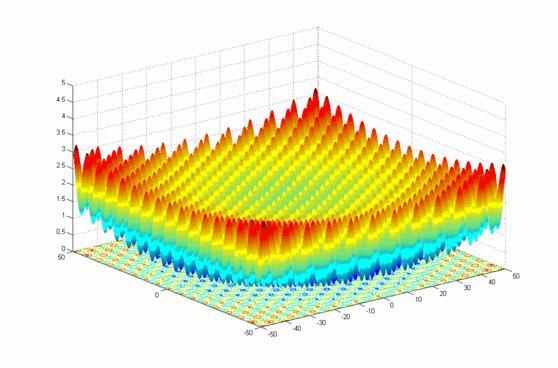
\includegraphics[scale=0.35]{griewank.jpg}
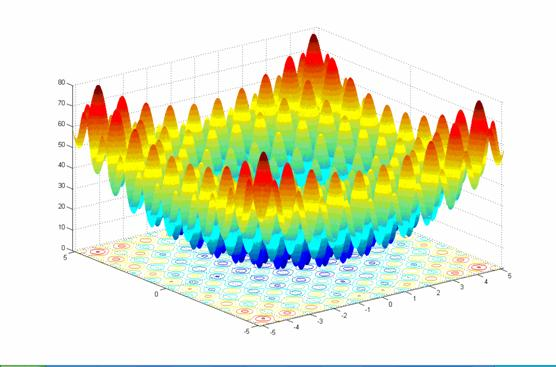
\includegraphics[scale=0.35]{Rastrigin.jpg}
\caption{Griewank \qquad \qquad \qquad \qquad \quad Rastrigin}
\end{figure}
\end{frame}

%------------------------------------------------

\begin{frame}
\frametitle{2 Ways for Smoothing}
\begin{itemize}
\item $\bar{f}(x)=f(x)+\frac{1}{6}\Delta^2trace(H)$  --- Trace-Smooth	
\item $\bar{f}(x)=f(x)+\lambda||x-x_*||_2^2$   --- $\lambda$-Smooth
\end{itemize}
Where $H$ is the Hessian matrix and $x_*$ is the global optimum we guess\\
$\Delta$ and $\lambda$ are defined by user\\
\end{frame}

%------------------------------------------------

\begin{frame}
\frametitle{Derivation of formula $\bar{f}(x)=f(x)+\frac{1}{6}\Delta^2trace(H)$}
Let $f$ be an objective function and $\Delta$ be a positive number. The average value of $f$ over a regular
$\Delta$-box $Box(x)$ centred at $x$ with sides $[x_i-\Delta ,x_i+\Delta ]$ is:
\begin{equation}\label{eq1}
\bar{f}(x)=\frac{1}{(2\ast\Delta)^n}\int_{Box(x)}f(x)dx_1...dx_n
\end{equation}
The formula above is too expensive to compute when $n$ is large or function $f$ is difficult to
compute. However, by approximating $f$ using quadratic Taylor series expansion
\begin{equation}
f(x+s)\cong f(x)+g^Ts+\frac{1}{2}s^THs\equiv q(x)
\end{equation}
where $g=\triangledown f(x)$,$H=\triangledown^2f(x)$ , (\ref{eq1}) can be approximated as
\begin{equation}
\bar{f}(x)\cong \bar{q}(x)=f(x)+\frac{1}{(2\ast\Delta)^n}\int_{\forall i,|s_i|\leq\Delta}(g^Ts+\frac{1}{2}s^THs)ds_1...ds_n
\end{equation}
\end{frame}

%------------------------------------------------

\begin{frame}
\frametitle{Continued}
Since $g^Ts+\frac{1}{2}s^THs=\sum_ig_is_i+\frac{1}{2}\sum_i\sum_js_is_jh_{ij}$. \\
Interchanging the order of summation and integration of the above formula yields:
\begin{equation}
\bar{f}(x)=f(x)+\frac{1}{6}\Delta^2\cdot trace(H)
\end{equation}
\end{frame}

%------------------------------------------------

\begin{frame}
\begin{figure}
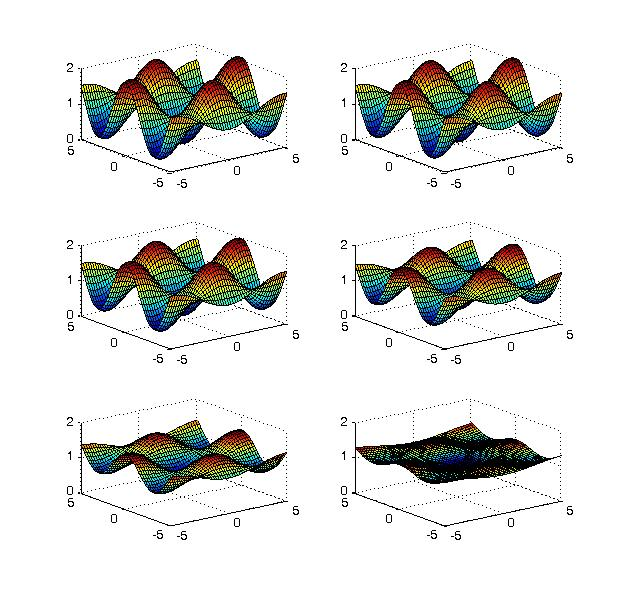
\includegraphics[scale=0.32]{smoothgriewank.jpg}
\caption{Griewank. $f(x)=\sum_{i=1}^n\frac{x_i^2}{4000}-\prod_{i=1}^n(\frac{x_i}{\sqrt{i}})+1$}
\end{figure}
\end{frame}

%------------------------------------------------

\begin{frame}
\begin{figure}
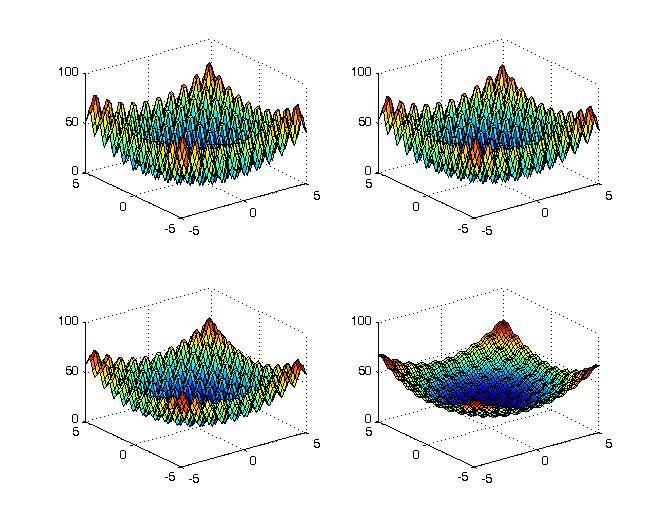
\includegraphics[scale=0.37]{smoothrast.jpg}
\caption{Rastrigin. $f(x)=10n+\sum_{i=1}^n(x_i^2-10\cos(2\pi x_i))$}
\end{figure}
\end{frame}

%------------------------------------------------

\begin{frame}
\begin{figure}
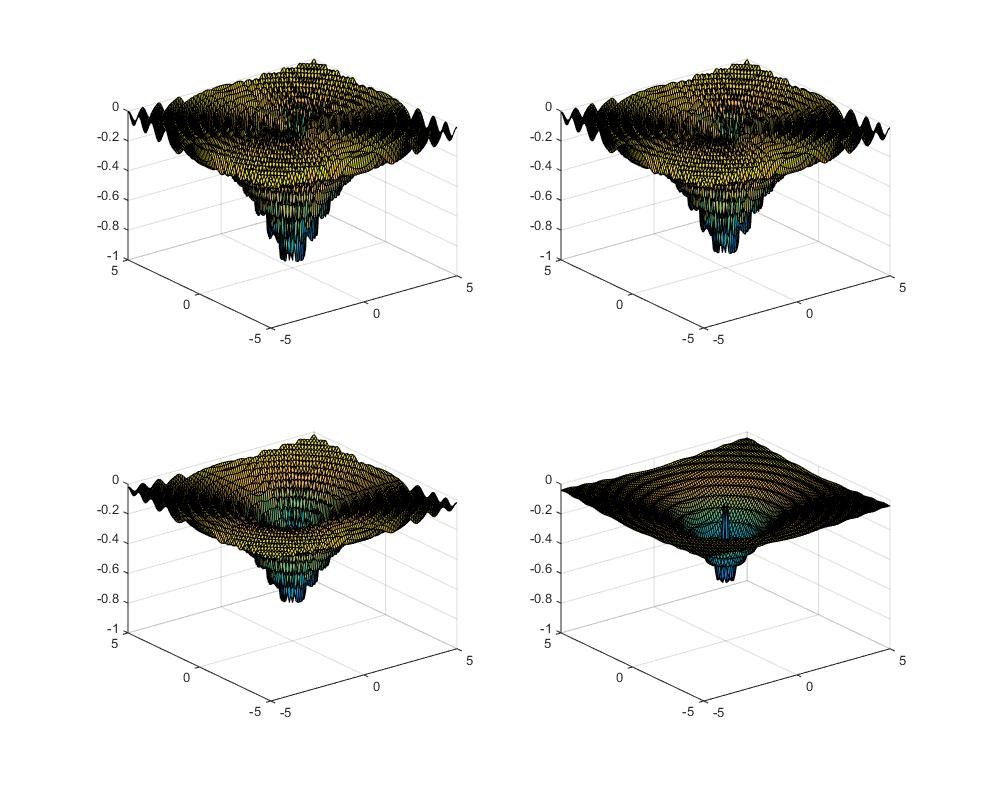
\includegraphics[scale=0.24]{dropsmooth.jpg}
\caption{Drop Wave. $f(x)=-\frac{1+\cos(12\sqrt{x_1^2+x_2^2})}{0.5(x_1^2+x_2^2)+2}$}
\end{figure}
\end{frame}

%------------------------------------------------

\begin{frame}
\begin{figure}
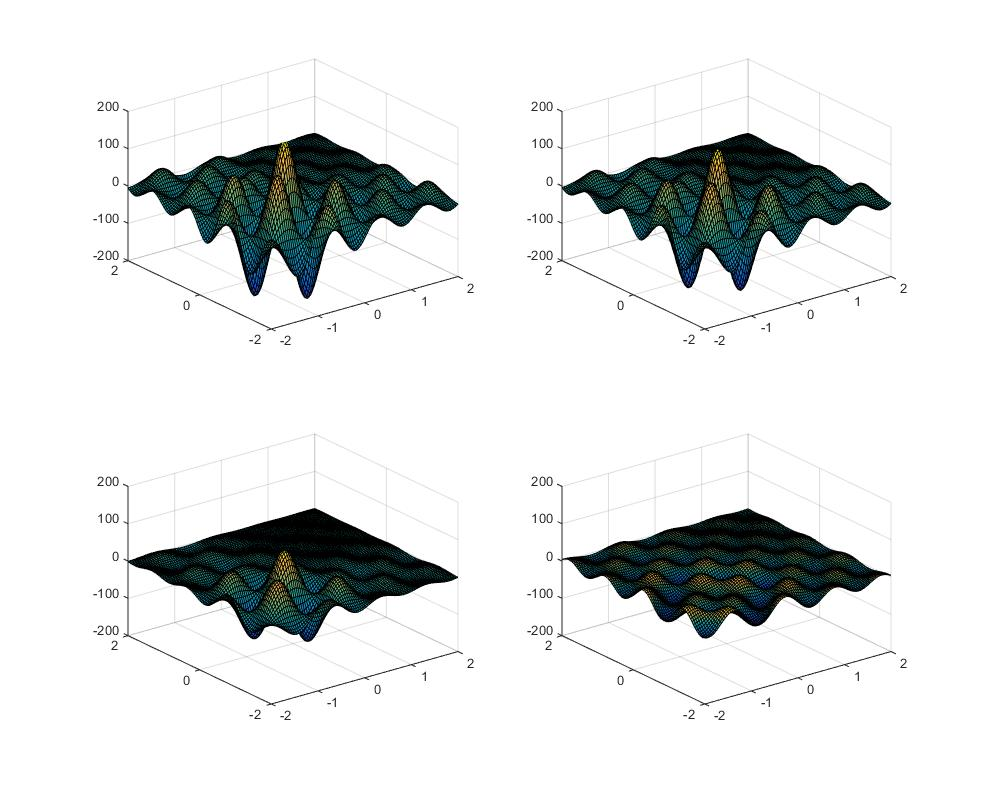
\includegraphics[scale=0.24]{shubertsmooth.jpg}\\
Shubert.$f(x)=(\sum_{i=1}^5i\cos((i+1)x_1+i))(\sum_{i=1}^5i\cos((i+1)x_2+i))$
\end{figure}
\end{frame}

%------------------------------------------------

\begin{frame}
\frametitle{Simulated Annealing Combined with Smoothing}
\begin{itemize}
\item We have $\Delta$-sequence or $\lambda$-sequence which contains several elements and the last one is 0. 
\item For each element of the smooth sequence, we run through all the temperatures using simulated annealing 
\end{itemize}
\end{frame}

%------------------------------------------------

\begin{frame}
\frametitle{Trust-Region Combined with Simulated Annealing and Smoothing}
\begin{itemize}
\item Traditional trust region only accept a point when the new point's value is less than current point. The main idea of trust-region combined with simulated annealing is that we accept a point when it decreases the function value $OR$ it increases the function value with a probability. 
\item Also, we can combine the Trust-Region with the smoothing technique
\end{itemize}
\end{frame}

%------------------------------------------------
\subsection{Numerical Results}
%------------------------------------------------

\begin{frame}
\begin{figure}
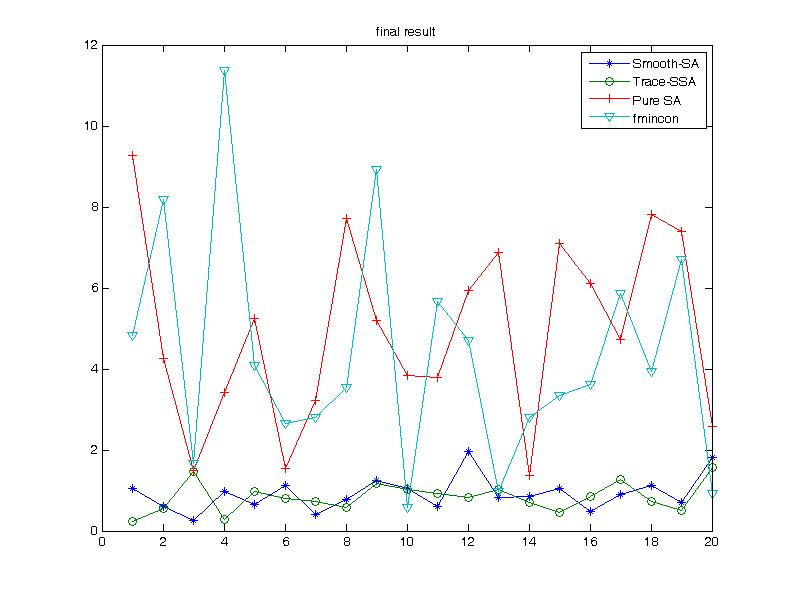
\includegraphics[scale=0.33]{result1.jpg}
\caption{Griewank $n=10$}
\end{figure}
\end{frame}

%------------------------------------------------

\begin{frame}
\begin{figure}
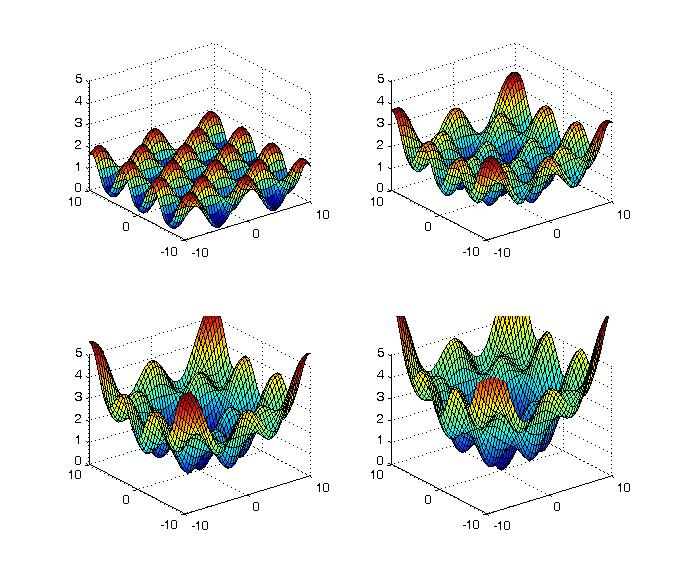
\includegraphics[scale=0.33]{diffp.jpg}
\caption{Griewank in different shape}
\end{figure}
\end{frame}

%------------------------------------------------

\begin{frame}
\begin{figure}
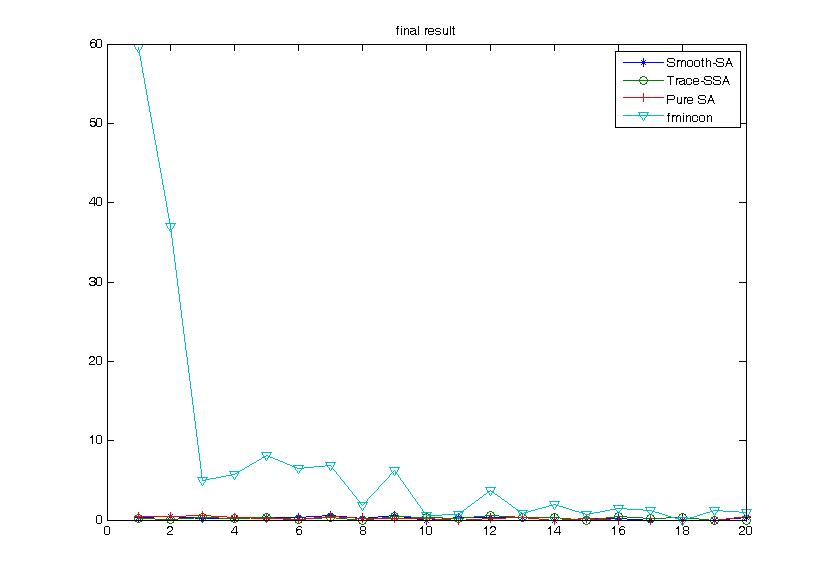
\includegraphics[scale=0.3]{result2.jpg}
\end{figure}
As $n$ goes bigger, the function become more and more flattened
\end{frame}

%------------------------------------------------

\begin{frame}
\begin{figure}
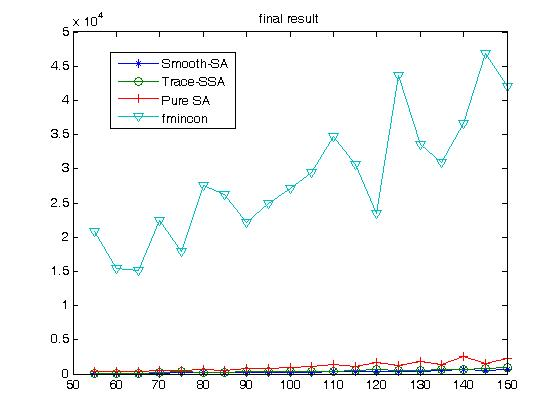
\includegraphics[scale=0.45]{result4.jpg}
\caption{Rastrigin. Compared with fmincon}
\end{figure}
\end{frame}

%------------------------------------------------

\begin{frame}
\begin{figure}
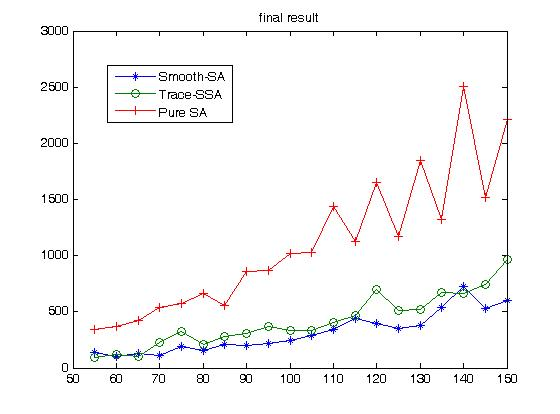
\includegraphics[scale=0.45]{result5.jpg}
\caption{Rastrigin. Remove fmincon}
\end{figure}
\end{frame}

%------------------------------------------------

\begin{frame}
\begin{figure}
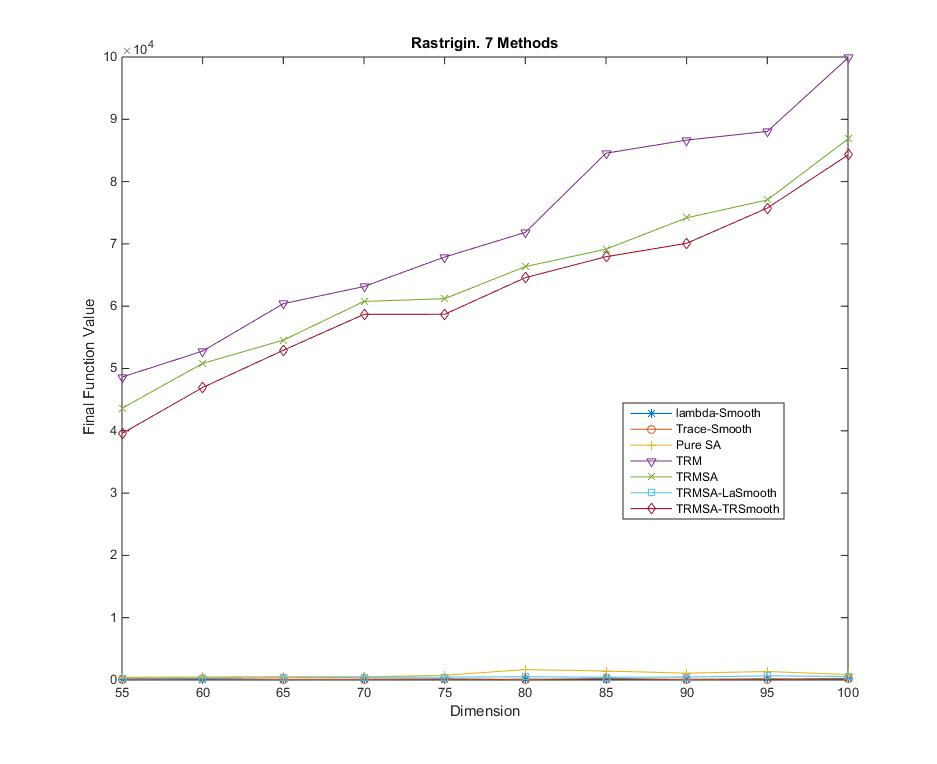
\includegraphics[scale=0.26]{result6.jpg}
\caption{Rastrigin. 7 Methods}
\end{figure}
\end{frame}

%------------------------------------------------

\begin{frame}
For $Trace-Smooth$ $\bar{f}(x)=f(x)+\frac{1}{6}\Delta^2trace(H)$, since $trace(H)=\sum_{i=1}^n\frac{\partial^2 f}{\partial x_i^2}$. So we have:
\begin{equation}
\bar{g}=g+\frac{1}{6}\Delta^2\frac{\partial^3 f}{\partial x^3}, \qquad
\bar{H}=H+\frac{1}{6}\Delta^2diag(\frac{\partial^4 f}{\partial x^4})
\end{equation} 

Where $g$ and $H$ is the gradient and Hessian matrix of original function $f(x)$ and 
\begin{equation}
\frac{\partial^3 f}{\partial x^3}=\left[ \begin{array}{c}
\frac{\partial^3 f}{\partial x_1^3}\\ \frac{\partial^3 f}{\partial x_2^3}\\ \cdots \\ \frac{\partial^3 f}{\partial x_n^3}
\end{array} \right], 
diag(\frac{\partial^4 f}{\partial x^4})=\left[ \begin{array}{cccc}
\frac{\partial^4 f}{\partial x_1^4} & 0 & \cdots & 0 \\
0 & \frac{\partial^4 f}{\partial x_2^4} & \cdots & 0 \\
\vdots & \vdots & \ddots & \vdots \\
0 & 0 & \cdots & \frac{\partial^4 f}{\partial x_n^4}
\end{array} \right]
\end{equation}
\end{frame}

\begin{frame}
\begin{figure}
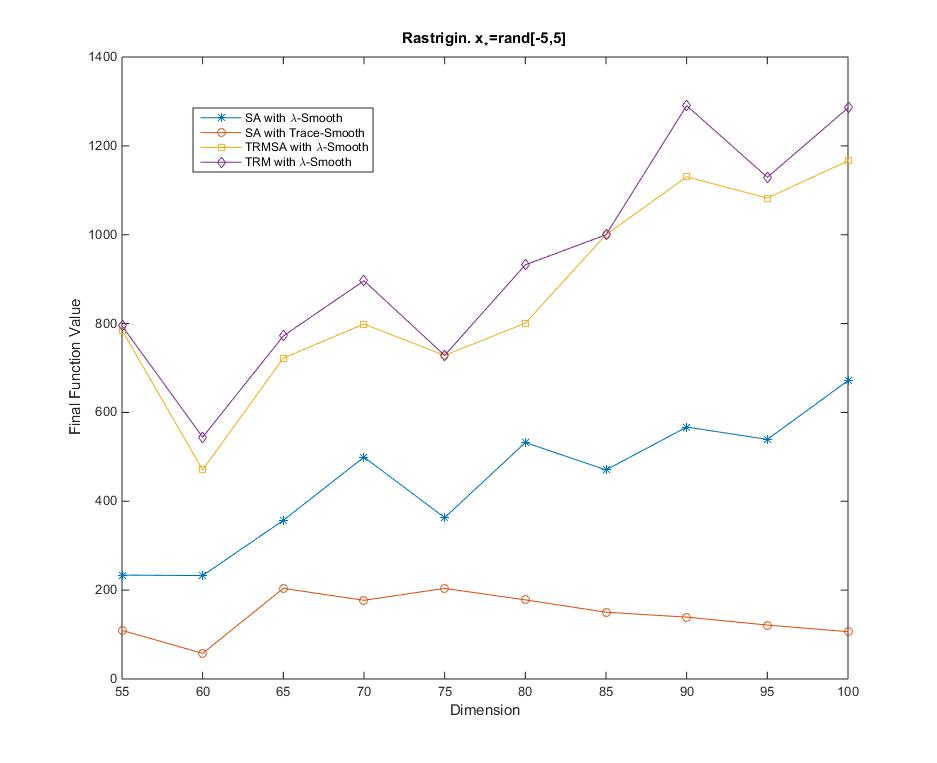
\includegraphics[scale=0.25]{result7.jpg}
\caption{Rastrigin. 4 Modified Methods}
\end{figure}
\end{frame}

%------------------------------------------------

\begin{frame}
\frametitle{Number of Evaluation of Function Value and Hessian Matrix}
\begin{tabular}{c c c c c}
 Dim  &   SAwithLa   &     SAwithTr    &  TRMSAwithLa  &   TRMwithLa  \\ \hline
  55  &  80412    0  &  80414   80412  &  3576   3575  &   627    626 \\
  60  &  80415    0  &  80412   80410  &  3152   3151  &  1116   1115 \\
  65  &  80412    0  &  80413   80411  &  3149   3148  &  1597   1596 \\
  70  &  80414    0  &  80418   80416  &  3528   3527  &   647    646 \\
  75  &  80416    0  &  80415   80413  &  3079   3078  &  1110   1109 \\
  80  &  80415    0  &  80416   80414  &  4533   4532  &   610    609 \\
  85  &  80413    0  &  80413   80411  &  3189   3188  &   679    678 \\
  90  &  80416    0  &  80415   80413  &  3522   3521  &   664    663 \\
  95  &  80418    0  &  80415   80413  &  3565   3564  &   671    670 \\
 100  &  80418    0  &  80417   80415  &  3287   3286  &  1605   1604 

\end{tabular}
\end{frame}

%------------------------------------------------
\section{Derivative Free Optimization}
%------------------------------------------------

%------------------------------------------------
\subsection{Introduction}
%------------------------------------------------

\begin{frame}
\frametitle{Motivation}
\begin{itemize}
\item In some cases, we can not get the derivative information and it takes very long to evaluate the function value. So it's impossible to use finite difference to evaluate the first and second derivative. 
\item Since the function is very expensive to compute, it is not ideal to use simulated annealing to optimize.
\end{itemize}
\end{frame}

%------------------------------------------------

\begin{frame}
\frametitle{Main Idea of DFO}
\begin{itemize}
\item We have a bunch of points and their function value to start. Use these points to build a model to approximate the original function, use this model to solve the optimization problem. We can update the model while solving the problem once we have more information about the function.
\item After we have the model, we can use trust-region or other methods to solve the problem.
\end{itemize}
\end{frame}

%------------------------------------------------

\begin{frame}
\frametitle{Choice of Model}
\begin{itemize}
\item There are many types of model we can choose to approximate the original function. We test two groups of them: Lagrange Polynomial Interpolation(LPI) and Radial Basis Function(RBF).
\end{itemize}
\end{frame}

%------------------------------------------------

\begin{frame}
\frametitle{Lagrange Polynomial Interpolation}
\begin{itemize}
\item Linear Model:
\begin{equation}
L(x)=\sum_{i=1}^na_ix_i+c
\end{equation}
\item Quadratic Model:
\begin{equation}
L(x)=\sum_{i=1}^n\sum_{j=i}^nb_{ij}x_ix_j+\sum_{i=1}^na_ix_i+c
\end{equation}
\end{itemize}
\end{frame}

%------------------------------------------------

\begin{frame}
\frametitle{Lagrange Polynomial Interpolation}
\begin{itemize}
\item We use $m$ points: $x_1, x_2,...,x_m$ and $f_1, f_2, ..., f_m$ to build the model $L(x)$.
\item $L(x)$ should satisfy $L(x_i)=f_i$, $i=1,...,m$.
\item In order to make the model unique, we need $n+1$ points to build the linear model and $\frac{(n+1)n}{2}+1$ points to build the quadratic model.
\end{itemize}
\end{frame}

%------------------------------------------------

\begin{frame}
\frametitle{Radial Basis Function}
\begin{itemize}
\item The model has the form:
\begin{equation}
R_m(x)=\sum_{i=1}^m\lambda_i\phi(||x-x_i||)+p(x)
\end{equation}
\item And we have different choices for $\phi(r)$ and $p(x)$:\\
\begin{center}
\begin{tabular}{l c r}
RBF & $\phi(r)>0$ & $p(x)$ \\ \hline
cubic & $r^3$ & $b^T\cdot x+a$ \\
linear & $r$ & $a$ \\
multiquadric & $(r^2+\gamma^2)^{\frac{1}{2}},\gamma>0$ & $a$ \\
Gaussian & $exp(-\gamma r^2),\gamma>0$ & $\{0\}$ 
\end{tabular}
\end{center}
\end{itemize}
\end{frame}

\begin{frame}
 To get the parameters $\lambda_i$, $b$, $a$ we need to solve the linear equations:
\begin{equation}
\left( \begin{array}{cc} \Phi & P \\
P^T & 0  \end{array} \right)
\left( \begin{array}{c} \lambda \\
c  \end{array} \right)
=
\left( \begin{array}{c} F \\
0  \end{array} \right)
\end{equation}

where $\Phi$ is the $m \times m$ matrix with $\Phi_{ij}=\phi(||x_i-x_j||)$ and
\begin{equation}
P=\left( \begin{array}{cc} x_1^T & 1 \\
x_2^T & 1  \\
\vdots & \vdots \\
x_m^T & 1 \end{array} \right),  
\lambda=\left( \begin{array}{c} \lambda_1 \\
\lambda_2  \\
\vdots  \\
\lambda_m \end{array} \right), 
c=\left( \begin{array}{c} b_1 \\
b_2  \\
\vdots  \\
b_n \\
a \end{array} \right),
F= \left( \begin{array}{c} f(x_1) \\
f(x_2)  \\
\vdots  \\
f(x_m) \end{array} \right).
\end{equation}
\end{frame}

%------------------------------------------------

\begin{frame}
\frametitle{Radial Basis Function}
\begin{itemize}
\item Notice that if we use a linear model for $p(x)$ and $rank(P)=n+1$, then the system has a unique solution.
\item Otherwise if we just use $p(x)=a$ or $p(x)=0$, then the system has a unique solution no matter how many points we have.
\item Also, it has different $\phi$ to choose.
\end{itemize}
\end{frame}

%------------------------------------------------
\subsection{Numerical Results}
%------------------------------------------------

\begin{frame}
\begin{figure}
\includegraphics[scale=0.25]{rbf1.jpg}
\caption{Radial Basis Function Approximation}
\end{figure}
\end{frame}

%------------------------------------------------

\begin{frame}
\begin{figure}
\includegraphics[scale=0.43]{rbf2.jpg}\\
Shubert.$f(x)=(\sum_{i=1}^5i\cos((i+1)x_1+i))(\sum_{i=1}^5i\cos((i+1)x_2+i))$
\end{figure}
\end{frame}

%------------------------------------------------

\begin{frame}[plain]
\begin{figure}
\includegraphics[scale=0.26]{rbf3.jpg}
\includegraphics[scale=0.26]{rbf4.jpg}\\
\includegraphics[scale=0.26]{rbf5.jpg}
\includegraphics[scale=0.26]{rbf6.jpg}
\end{figure}
\end{frame}

%------------------------------------------------

\begin{frame}
\frametitle{Radial Basis Function}
\begin{itemize}
\item Once we have built the model $R_m(x)$, we can easily compute the derivative:
\begin{equation}
R_m'(x)=\sum_{i=1}^m\lambda_i\phi'(||z_i||)\frac{z_i}{||z_i||}+p'(x)
\end{equation}
and
\begin{equation}
R_m''(x)=\sum_{i=1}^m\lambda_i\left[\frac{\phi'(||z_i||)}{||z_i||}I_n+\{\phi''(||z_i||)-\frac{\phi'(||z_i||)}{||z_i||}\} \frac{(z_i)(z_i)^T}{||z_i||^2}\right]
\end{equation}
$z_i=x-x_i$
\end{itemize}
\end{frame}

%------------------------------------------------

\begin{frame}
\begin{figure}
\includegraphics[scale=0.26]{rbfr1.jpg}
\end{figure}
\end{frame}

%------------------------------------------------

\begin{frame}
\begin{figure}
\includegraphics[scale=0.26]{rbfr2.jpg}
\end{figure}
\end{frame}

%------------------------------------------------

\begin{frame}
\begin{figure}
\includegraphics[scale=0.26]{rbfr3.jpg}
\end{figure}
\end{frame}

%------------------------------------------------

\begin{frame}
\begin{figure}
\includegraphics[scale=0.26]{rbfr4.jpg}
\end{figure}
\end{frame}


%------------------------------------------------
\section{Summary}
%------------------------------------------------

%------------------------------------------------
\subsection{Summary}
%------------------------------------------------

\begin{frame}
\frametitle{TRM, SA, DFO and Smoothing}
\begin{itemize}
\item Each method has its own advantages and disadvantages.
\item Our new methods work more efficiently than the traditional ways.
\end{itemize}
\end{frame}

%------------------------------------------------

\begin{frame}
\frametitle{Challenge}
\begin{itemize}
\item $\Delta$ for Trace-Smoothing is really important for the method, but it's a little difficult to find it perfect cause it depends on the problem.
\item The $\lambda$ smooth technique can work well in the condition that we know where the global optimum locates.
\item If the search region is quite big, the RBF may not approximate the original function very well just use several points.
\end{itemize}
\end{frame}

%------------------------------------------------

\begin{frame}
\frametitle{Further work}
\begin{itemize}
\item Need more examples and test problems.
\item How to decide the parameters and the models.
\end{itemize}
\end{frame}

%------------------------------------------------
\subsection{Reference}
%------------------------------------------------

\begin{frame}
\frametitle{Reference}
\begin{itemize}
\item \url{http://www.sfu.ca/~ssurjano/optimization.html}
\item \url{http://www.mcs.anl.gov/~wild/orbit/}
\item \url{https://courses.cit.cornell.edu/jmueller/}
\item ORBIT: Optimization by Radial Basis Function Interpolation in Trust-Regions
\item Introduction to Derivative-Free Optimization
\end{itemize}
\end{frame}

%------------------------------------------------

\begin{frame}
\Huge{\centerline{Thanks}}
\end{frame}

%----------------------------------------------------------------------------------------

\end{document} 